\documentclass[11pt]{article}

%%%%%%%%%%%%
% Packages %
%%%%%%%%%%%%

\hyphenpenalty=10000
\usepackage{tikz}
\usetikzlibrary{shapes,arrows}

\usepackage{tocloft}
\renewcommand\cftsecleader{\cftdotfill{\cftdotsep}}
\def\undertilde#1{\mathord{\vtop{\ialign{##\crcr
$\hfil\displaystyle{#1}\hfil$\crcr\noalign{\kern1.5pt\nointerlineskip}
$\hfil\tilde{}\hfil$\crcr\noalign{\kern1.5pt}}}}}
\usepackage{cleveref}
\usepackage{xcolor}
\usepackage[colorlinks = true,
            linkcolor = black,
            urlcolor  = black,
            citecolor = black,
            anchorcolor = black]{hyperref}
\usepackage{epstopdf}
\usepackage{braket}
\usepackage{upgreek}
\usepackage{caption}
\usepackage{booktabs}
\usepackage{subcaption}
\usepackage{amssymb,latexsym,amsmath,gensymb}
\usepackage{latexsym}
\usepackage{graphicx}
\usepackage{float}
\usepackage{enumitem}
\usepackage{pdflscape}
\usepackage{url}
\usepackage{array}
\newcolumntype{C}{>{$\displaystyle} c <{$}}
\usepackage{tikz, calc}
\usetikzlibrary{shapes.geometric, arrows, calc}
\tikzstyle{norm} = [rectangle, rounded corners, minimum width=2cm, minimum height=1cm,text centered, draw=black]
\tikzstyle{arrow} = [thick, ->, >=stealth]

\newcommand{\argmin}{\arg\!\min}
\newcommand{\me}{\mathrm{e}}
\providecommand{\e}[1]{\ensuremath{\times 10^{#1}}} 
\providecommand{\mb}[1]{\mathbf{#1}}
\providecommand{\mf}[1]{\mathbf{#1}}
\providecommand{\ro}[1]{\mathbf{\mathbf{r}}_o}
\providecommand{\so}[1]{\mathbf{\hat{s}}_o}
\providecommand{\rb}[1]{\mathbf{r}_b}
\providecommand{\rbm}[1]{r_b^{\text{m}}}
\providecommand{\rd}[1]{\mathbf{r}_d}
\providecommand{\mh}[1]{\mathbf{\hat{#1}}}
\providecommand{\bs}[1]{\boldsymbol{#1}} 
\providecommand{\intinf}{\int_{-\infty}^{\infty}}
\providecommand{\fig}[4]{
  % filename, width, caption, label
\begin{figure}[h]
 \captionsetup{width=1.0\linewidth}
 \centering
 \includegraphics[width = #2\textwidth]{#1}
 \caption{#3}
 \label{fig:#4}
\end{figure}
}

\newcommand{\tensor}[1]{\overset{\text{\tiny$\leftrightarrow$}}{\mb{#1}}}
\newcommand{\tunderbrace}[2]{\underbrace{#1}_{\textstyle#2}}
\providecommand{\figs}[7]{
  % filename1, filename2, caption1, caption2, label1, label2, shift
\begin{figure}[H]
\centering
\begin{minipage}[b]{.45\textwidth}
  \centering
  \includegraphics[width=1.0\linewidth]{#1}
  \captionsetup{justification=justified, singlelinecheck=true}
  \caption{#3}
  \label{fig:#5}
\end{minipage}
\hspace{2em}
\begin{minipage}[b]{.45\textwidth}
  \centering
  \includegraphics[width=1.0\linewidth]{#2}
  \vspace{#7em}
  \captionsetup{justification=justified}
  \caption{#4}
  \label{fig:#6}
\end{minipage}
\end{figure}
}
\makeatletter

\providecommand{\code}[1]{
\begin{center}
\lstinputlisting{#1}
\end{center}
}

\newcommand{\crefrangeconjunction}{--}
%%%%%%%%%%%
% Spacing %
%%%%%%%%%%%
% Margins
\usepackage[
top    = 1.5cm,
bottom = 1.5cm,
left   = 1.5cm,
right  = 1.5cm]{geometry}

% Indents, paragraph space
%\usepackage{parskip}
\setlength{\parskip}{1.5ex}

% Section spacing
\usepackage{titlesec}
\titlespacing*{\title}
{0pt}{0ex}{0ex}
\titlespacing*{\section}
{0pt}{0ex}{0ex}
\titlespacing*{\subsection}
{0pt}{0ex}{0ex}
\titlespacing*{\subsubsection}
{0pt}{0ex}{0ex}

% Line spacing
\linespread{1.1}

%%%%%%%%%%%%
% Document %
%%%%%%%%%%%%
\begin{document}
\title{\vspace{-2.5em} Spatio-angular transfer functions for fluorescence microscopes\vspace{-1em}}  \author{Talon Chandler, Min Guo, Hari Shroff, Rudolf Oldenbourg, Patrick La Rivi\`ere}
\date{\vspace{-1em}\today\vspace{-1em}}
\maketitle
\begin{abstract}
  We investigate how the orientation and position of fluorescent dipole emitters
  affects microscopic imaging using electromagnetic optics theory. Starting with
  the thoroughly studied spatio-angular point spread function, we introduce the
  spatio-angular coherent spread function, coherent transfer function, and
  optical transfer function as electromagnetic extensions of well-known
  functions in scalar optics theory. We use these concepts to show that
  fluorescence microscopes have a spatio-angular band limit. Finally, we study
  polarized light microscopes and find that polarized illumination is a type of
  structured illumination that extends the angular band limit.
\end{abstract}
\section{Introduction}
TODO

We use plain roman type for scalars, e.g., $x, y, z$; bold lowercase roman type
for two-dimensional vectors, e.g., $\mb{r}$; hats for unit vectors, e.g.,
$\mb{\hat{s}}$; and bold capital roman type for matrices, e.g.,
$\mb{R}$. We use the real spherical harmonic functions
\begin{align}
  y_l^m(\vartheta, \varphi) =
  \begin{cases}
    \sqrt{2}K_l^m\cos(m\varphi)P_l^m(\cos\vartheta), & m > 0\\
    K_l^0P_l^0(\cos\vartheta), & m = 0\\
    \sqrt{2}K_l^m\sin(-m\varphi)P_l^{-m}(\cos\vartheta), & m < 0\\
  \end{cases}
\end{align}
where
\begin{align}
  K_l^m = \sqrt{\frac{(2l+1)}{4\pi}\frac{(l-|m|)!}{(l+|m|)!}},
\end{align}
and $P_l^m(x)$ are the associated Legendre polynomials. The $l=0$ and $l=1$
spherical harmonics are given by
\begin{equation}
\begin{aligned}
  y_0^0(\vartheta, \varphi) &= \sqrt{\frac{1}{4\pi}},\\
  y_1^{-1}(\vartheta, \varphi) = \sqrt{\frac{3}{4\pi}}\sin\varphi\sin\vartheta, \hspace{2em} y_1^0(\vartheta, \varphi) &= \sqrt{\frac{3}{4\pi}}\cos\vartheta, \hspace{2em} y_1^1(\vartheta, \varphi) = \sqrt{\frac{3}{4\pi}}\cos\varphi\sin\vartheta. \label{eq:harmonics}
\end{aligned}
\end{equation}

\section{Spatio-angular point spread functions}
\begin{figure}[h]
 \captionsetup{width=1.0\linewidth}
 \centering
   \centering
   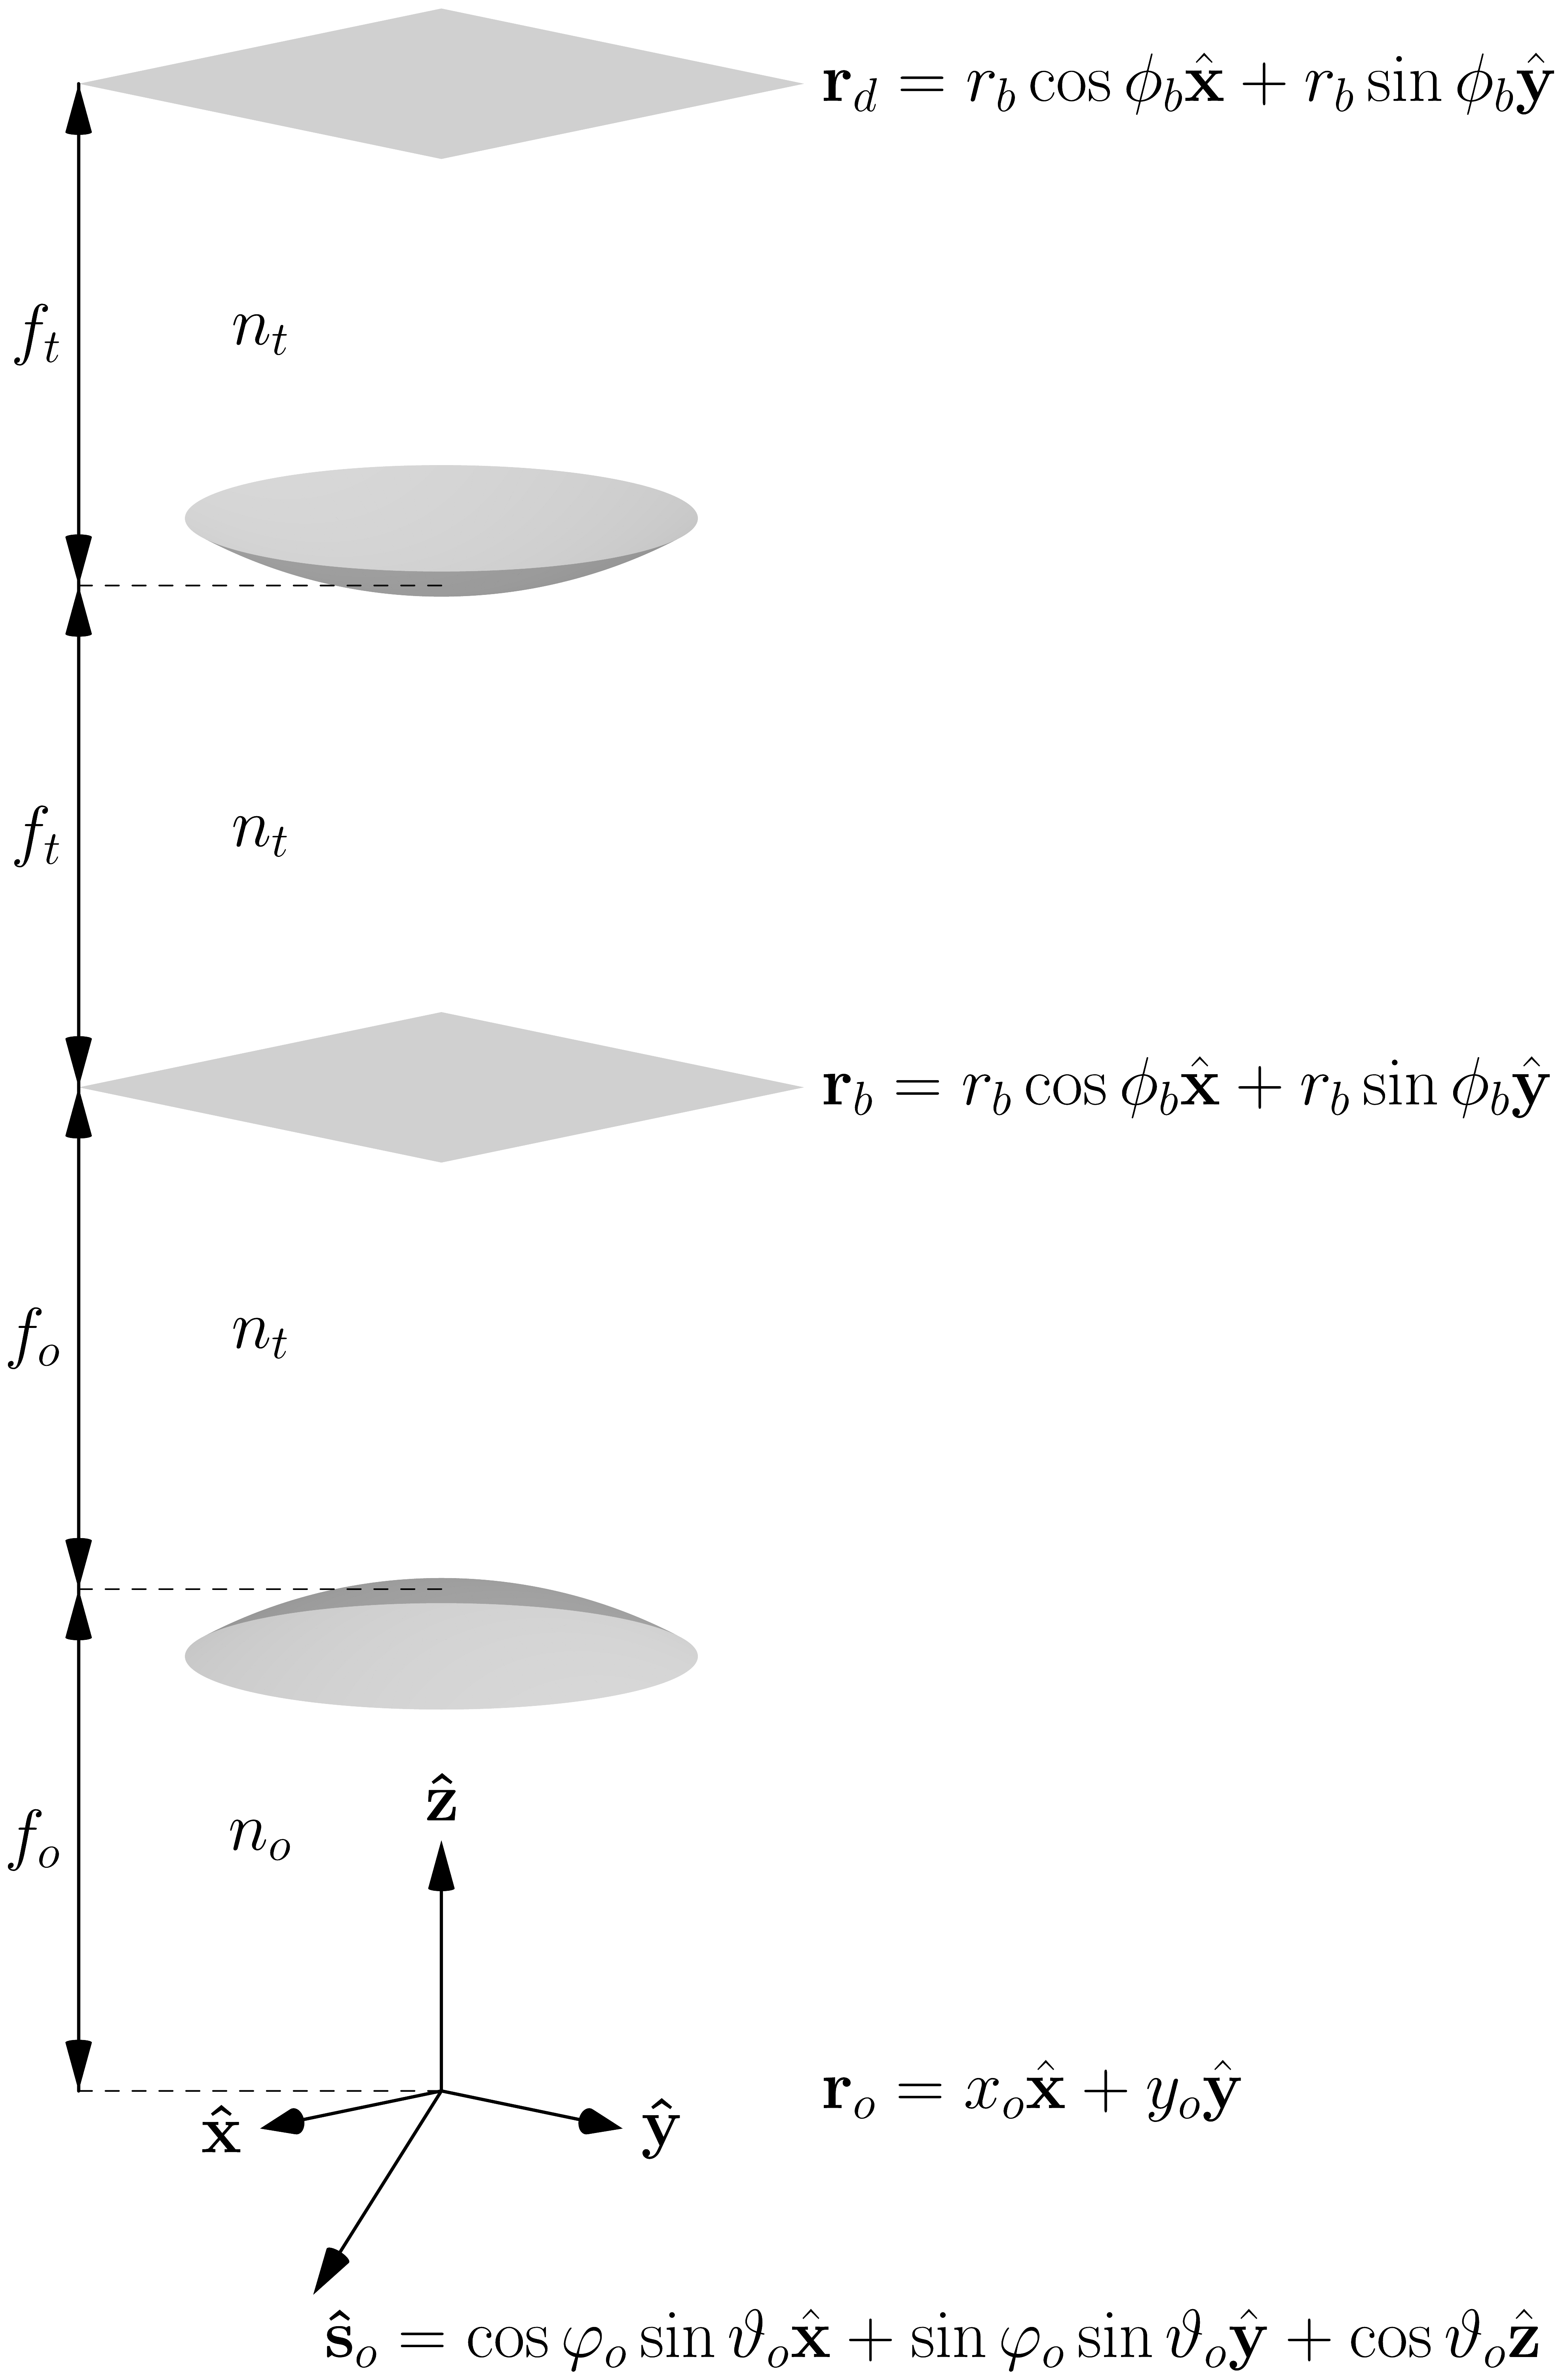
\includegraphics[width = 0.4\textwidth]{../figures/schematic.pdf}
   \caption{Simplified schematic of a single-view fluorescence microscope. The
     object is placed near the focal point of an aplanatic objective lens with
     focal length $f_{o}$ in a medium with refractive index $n_o$. The object is
     parameterized by the 2D position vector $\ro{}$ ($o$ for object) and an
     orientation unit vector $\so{}$. The light emitted by the fluorescent
     object is collected and collimated by the objective lens so that the
     electric fields are purely transverse in the back focal plane. Points in
     the back focal plane are parameterized by a 2D position vector $\rb{}$ ($b$
     for back focal plane). Finally, the tube lens with focal length $f_t$
     refocuses the light onto a detector. Points on the detector are
     parameterized by a 2D position vector $\rd{}$ ($d$ for detector). The back
     focal plane and detector are in a medium with refractive index $n_t$. Note
     that this schematic is not to scale---we consider the case where
     $f_o \ll f_t$.}
   \label{fig:frames_a}
\end{figure}

Figure \ref{fig:frames_a} shows a schematic of the fluorescence microscope that
we are considering with a summary of our notation. We start by following Backer
and Moerner \cite{backer2014} to find the electric field at position $\rb{}$ in
the back focal plane due to a single dipole emitter at position $\ro{}$ oriented
along $\so{}$ as
\begin{align}
  \mb{\tilde{e}}_b(\rb{};\ro{}, \so{}) \propto \me^{-i(kn_o/f_o)\rb{}\cdot\ro{}}\sqrt{\frac{1}{\rho_b}}
  \begin{bmatrix}
    \sin^2\phi_b + \rho_b\cos^2\phi_b&\sin\phi_b\cos\phi_b(\rho_b - 1)&-\frac{r_b}{f_o}\cos\phi_b\\
    \sin\phi_b\cos\phi_b(\rho_b - 1)&\cos^2\phi_b + \rho_b\sin^2\phi_b&-\frac{r_b}{f_o}\sin\phi_b\\
    0&0&0
  \end{bmatrix}
  \begin{bmatrix}
    \cos\varphi_o\sin\vartheta_o\\
    \sin\varphi_o\sin\vartheta_o\\
    \cos\vartheta_o
  \end{bmatrix}
\Pi\left(\frac{r_b}{r_b^{\text{max}}}\right)\label{eq:bfp}
\end{align}
where we define $\rho_b \equiv \sqrt{1 - \left(\frac{r_b}{f_o}\right)^2}$, and
$\Pi(x)$ is a boxcar function that returns 1 when $|x| < 1$ and 0 otherwise. We
can understand this expression term by term---the exponential term accounts for
the phase as dipole emitter is moved in object space, the square root term
conserves power before and after the objective lens, the matrix models the
dipole emission process and electric field rotation caused by the objective
lens, the vector is the dipole orientation unit vector, and
$\Pi\left(\frac{r_b}{r_b^{\text{max}}}\right)$ accounts for the numerical
aperture of the lens with $r_b^{\text{max}} = \frac{f_0}{n_0}\text{NA}$. We use
a tilde to mark single dipole response functions---we will consider the response
due to a field of dipoles in the next section.

Although we will not use the result immediately, we can write the electric field
in back focal plane under the paraxial approximation. We expand Eq. \ref{eq:bfp}
in a Taylor series about $r_b=0$ and drop all second-order and higher terms to
find
\begin{align}
  \mb{\tilde{e}}^{(p)}_b(\rb{};\ro{}, \so{}) \propto \me^{-i(kn_o/f_o)\rb{}\cdot\ro{}}
  \begin{bmatrix}
    1 & 0 &-\frac{r_b}{f_o}\cos\phi_b\\
    0&1&-\frac{r_b}{f_o}\sin\phi_b\\
    0&0&0
  \end{bmatrix}
  \begin{bmatrix}
    \cos\varphi_o\sin\vartheta_o\\
    \sin\varphi_o\sin\vartheta_o\\
    \cos\vartheta_o
  \end{bmatrix}
\Pi\left(\frac{r_b}{r_b^{\text{max}}}\right)\label{eq:bfppara}
\end{align}
We will continue to use a superscript $(p)$ to mark terms that have used the
paraxial approximation.

If the tube lens is weakly focusing ($f_o \ll f_t$) then we can find the
electric field in the detector plane by taking the Fourier transform of the
electric field in the back focal plane
\begin{align}
  \mb{\tilde{e}}_d(\rd{}; \ro{}, \so{}) \propto \int_{\mathbb{R}^2} d\rb{}\, \tilde{\mb{e}}_b(\rb{}; \ro{}, \so{})\me^{-i (kn_t/f_t) \rb{} \cdot \rd{}}. \label{eq:ed}
\end{align}
By isolating the phase term in Eq. \ref{eq:bfp} with
$\mb{\tilde{e}}_b(\rb{};\ro{}, \so{}) \equiv \me^{-i(kn_o/f_o)\rb{}\cdot\ro{}}
\tilde{\underline{\mb{e}}}_b(\rb{};\so{})$, and plugging into Eq. \ref{eq:ed} we find
that 
\begin{align}
  \mb{\tilde{e}}_d(\rd{} - M\ro{}, \so{}) \propto \int_{\mathbb{R}^2} d\rb{}\, \tilde{\underline{\mb{e}}}_b(\rb{}; \so{})\me^{-i (kn_t/f_t)\, \rb{} \cdot [\,\rd{} - M\ro{}]}.
\end{align}
where $M = -\frac{n_o}{n_t}\frac{f_t}{f_o}$ is the transverse magnification.  By
writing the electric field in the detector plane in terms of $\rd{} - M\ro{}$,
we have established that the electric field in the detector plane is
\textit{transverse shift-invariant}---a transverse shift of the object creates a
magnified transverse shift of the image. We define coordinates on the detector
centered on the image of the object
$\rd{}' \equiv \rd{} - M\ro{} = r_d'\cos\phi_d'\mh{x} + r_d'\sin\phi_d'\mh{y}$,
then we follow Novotny \cite{nov2006} by writing the integrals in polar
coordinates, evaluating the azimuthal integrals, and writing the result
concisely in terms of three radial integrals
\begin{align}
  \tilde{\mb{e}}_d(\rd{}', \so{}) &\propto
  \begin{bmatrix}
    A(r_d') + C(r_d')\cos(2\phi_d') & C(r_d')\sin(2\phi_d') & 2iB(r_d')\cos\phi_d'\\
    C(r_d')\sin(2\phi_d') & A(r_d') - C(r_d')\cos(2\phi_d') & 2iB(r_d')\sin\phi_d'\\
    0&0&0\\
  \end{bmatrix}
  \begin{bmatrix}
    \cos\varphi_o\sin\vartheta_o\\
    \sin\varphi_o\sin\vartheta_o\\
    \cos\vartheta_o
  \end{bmatrix}\label{eq:elec}
\end{align}
where $A(r_d'), B(r_d')$, and $C(r_d')$ are
\begin{align}
  A(r_d') &= \int_0^{\theta_{\text{max}}}d\theta\ \sqrt{\cos\theta}\sin\theta(1+\cos\theta)J_0(k_b r_d'\sin\theta f_o/f_t),\\%\ \text{exp}\left\{ik_bz_o[1-(1/2)(f_o/f_t)^2\sin^2\theta]\right\},\\
  B(r_d') &= \int_0^{\theta_{\text{max}}}d\theta\ \sqrt{\cos\theta}\sin^2\theta J_1(k_b r_d'\sin\theta f_o/f_t),\\%\ \text{exp}\left\{ik_bz_o[1-(1/2)(f_o/f_t)^2\sin^2\theta]\right\},\\
  C(r_d') &= \int_0^{\theta_{\text{max}}}d\theta\ \sqrt{\cos\theta}\sin\theta(1-\cos\theta)J_2(k_b r_d'\sin\theta f_o/f_t).%\ \text{exp}\left\{ik_bz_o[1-(1/2)(f_o/f_t)^2\sin^2\theta]\right\}.
\end{align}
We can identify Eq. \ref{eq:elec} as the vector-valued \textit{coherent spread
  function} (CSF) of the microscope. The scalar-valued CSF---sometimes called
the amplitude transfer function---is only applicable to cases where
electromagnetic optics plays no role in the microscope---not true
for samples that contain dipole emitters. 

To build our intuition about the CSF, we will rewrite the matrix multiplication
in Eq. \ref{eq:elec} in terms of the spherical harmonics. Notice that the $l=1$
spherical harmonics are the Cartesian components of the unit dipole axis (see
Eq. \ref{eq:harmonics}), so the CSF becomes
\begin{align}
  \tilde{\mb{e}}_d(\rd{}', \so{}) &\propto
  \begin{bmatrix}
    [A(r_d') + C(r_d')\cos(2\phi_d')]y_1^{1}(\so{}) + C(r_d')\sin(2\phi_d')y_1^{-1}(\so{}) + 2iB(r_d')\cos\phi_d'y_1^{0}(\so{})\\
    C(r_d')\sin(2\phi_d')y_1^{1}(\so{}) + [A(r_d') - C(r_d')\cos(2\phi_d')]y_1^{-1}(\so{}) + 2iB(r_d')\sin\phi_d'y_1^{0}(\so{})\\
    0\\
  \end{bmatrix}.
\end{align}
By applying the paraxial approximation ($\sin\theta\approx\theta$ and
$\cos\theta\approx 1$), the integrals $A(r_d'), B(r_d')$ and $C(r_d')$ can be
evaluated in terms of Bessel functions. We can evaluate $A(r_d')$ and $B(r_d')$ with the
help of $\int_0^zdx\ xJ_0(ax) = zJ_1(az)/a$ and
$\int_0^zdx\ x^2J_1(ax) = z^2J_2(az)/a$, respectively, and $C(r_d') = 0$ because
$J_2(x)$ is zero to first order. In this case, the CSF simplifies to
\begin{align}
  \tilde{\mb{e}}^{(p)}_d(\rd{}', \so{}) &\propto
  \begin{bmatrix}
    A^{(p)}(r_d')y_1^{1}(\so{}) + 2iB^{(p)}(r_d')\cos\phi_d'y_1^{0}(\so{})\\
    A^{(p)}(r_d')y_1^{-1}(\so{}) + 2iB^{(p)}(r_d')\sin\phi_d'y_1^{0}(\so{})\\
    0\\
  \end{bmatrix}\label{eq:paracsf}
\end{align}
where the integrals evaluate to
\begin{align}
  {A^{(p)}}(r_d') = \frac{J_1(2\pi ar_d')}{\pi ar_d'}, 
  &\hspace{2em}
    {B^{(p)}}(r_d') = \frac{\text{NA}}{n_o}\left[\frac{J_2(2\pi ar_d')}{\pi ar_d'}\right],  \label{eq:abparadef}
  \intertext{and we have substituted}
  a \equiv \frac{\text{NA}}{M\lambda},&\hspace{2em}
  \text{NA} \equiv n_o\sin\theta_{\text{max}}.
\end{align}
Under the paraxial approximation the electric fields on the detector created by
a single dipole are composed of two parts, a parallel part and a radial
part. The coefficients of the $y_1^0$ spherical harmonic in Eq. \ref{eq:paracsf}
create the radial part of the field---the $z$ component of the dipole generates
a radial field on the detector with respect to the image point. The coefficients
of the $y_1^1$ and $y_1^{-1}$ spherical harmonics create a parallel field in the
detector plane parallel to the $x$ and $y$ components of the
dipole. As the NA increases and the paraxial approximation no longer applies, we
begin to see coupling between the $x(y)$ component of the dipole with the $y(x)$
transverse field.

We can find the intensity in the detector plane due to a single dipole
by taking the modulus squared of the CSF
\begin{align}
  h(\rd{}', \so{}) = \left|\tilde{\mb{e}}_d(\rd{}', \so{})\right|^2 \label{eq:kernel}.
\end{align}
For convenience we keep the CSF written in terms of the spherical harmonics and
use a table of spherical harmonic products (see Appendix \ref{realspherical}) to
calculate the intensity in the detector plane as
\begin{equation}
  \begin{split}
  h(\rd{}', \so{}) \propto &\left(A^2(r_d') + 2B^2(r_d') + C^2(r_d')\right)y_0^0(\so{}) -\frac{2\sqrt{15}}{5}A(r_d')C(r_d')\sin(2\phi_d')y_2^{-2}(\so{})\\ &+ \frac{1}{\sqrt{5}}\left(-A^2(r_d') + 4B^2(r_d') - C^2(r_d')\right)y_2^{0}(\so{}) +\frac{2\sqrt{15}}{5}A(r_d')C(r_d')\cos(2\phi_d')y_2^{2}(\so{}). \label{eq:kerna}
\end{split}
\end{equation}
We can identify Eq. \ref{eq:kerna} as the spatio-angular \textit{point spread
  function} (PSF) of the microscope. Writing the spatio-angular PSF in terms of
spherical harmonic functions has two advantages. First, it allows us to express
the spatio-angular PSF very concisely. Instead of considering the point spread
function for every possible dipole orientation, we only need to consider four
spatio-angular PSFs---one for each spherical harmonic. Second, the spherical
harmonic functions form an orthonormal basis for functions on the sphere---a
convenient fact that we will use later.

It is useful to compare Eq. \ref{eq:kerna} to Backer and Moerner's approach
\cite{backer2014}. They expand the spatio-angular PSF in terms of six second
moments of the fluorophore distribution
$\{s_x^2, s_y^2, s_z^2, s_xs_y, s_xs_z, s_ys_z\}$. This approach is very
useful---only six precomputed spatio-angular PSFs are required to represent an
arbitrary spatio-angular PSF. Instead of expanding in terms of six second
moments, we expand onto just four spherical harmonics which, unlike the second
moments, are orthonormal functions. In the next section we will use the
orthonormality of the spherical harmonics to derive spatio-angular transfer
functions for fluorescence microscopes.

The spatio-angular PSF under the paraxial approximation is given by
\begin{align}
      h^{(p)}(\rd{}', \so{}) \propto \left({A^{(p)}}^2(r_d') + 2{B^{(p)}}^2(r_d')\right)y_0^0(\so{}) + \frac{1}{\sqrt{5}}\left(-{A^{(p)}}^2(r_d') + 4{B^{(p)}}^2(r_d')\right)y_2^{0}(\so{})\label{eq:para}.
\end{align}
First, consider the coefficient on the $y_0^0$ spherical harmonic in Eq.
\ref{eq:para}. This coefficient is the point spread function for an angularly
uniform distribution of fluorophores. The first term of the coefficient
${A^{(p)}}^2(r_d')$ is the familiar Airy disk that arises from the contribution
of dipoles oriented in the transverse plane, while the second term
${B^{(p)}}^2(r_d')$ is a smaller factor that arises from dipoles oriented
outside of the transverse plane. This leads to an interesting conclusion---a
uniform distribution of dipoles has a point spread function that is slightly
wider than an Airy disk even in the paraxial approximation. The Airy disk is
usually derived using paraxial scalar optics while here we have used paraxial
electromagnetic optics. Therefore, we can consider the second term to be an
electromagnetic correction to the Airy disk. We will quantify this difference in
the next section.

Next, consider the coefficient on the $y_2^0$ spherical harmonic in
Eq. \ref{eq:para}. This coefficient is the spatial PSF for a distribution of
fluorophores proportional to $3\cos^2\vartheta_o - 1$. Counterintuitively, this
fluorophore distribution cannot exist because it would require a negative number
of fluorophores along some orientations; but if this distribution could exist,
then this coefficient would be its spatial PSF. Considering negative
distributions of fluorophores in our calculations should not be cause for
concern. The spherical harmonics span the space of functions on the sphere, so
any positive fluorophore distribution can be represented by the spherical
harmonics and we never need to consider negative fluorophores.
    
Finally, consider all of the spherical harmonics that have a zero
coefficient. These spherical harmonics span the angular null space of our
measurement system---fluorophore distributions that lie in the null space do not
affect the measured intensities. Under the paraxial approximation all of the
non-zero coefficients are rotationally symmetric ($m=0$) spherical harmonics
which means that the transverse orientation of the dipoles does not affect the
PSF. In the high NA case this is no longer true---two $m=2$ spherical harmonics
have non-zero coefficients and the transverse orientation of dipoles does affect
the PSF.


\section{Spatio-angular transfer functions}
Consider a thin object that consists of fluorescent dipoles in arbitrary
positions and orientations. We can represent the entire object using a function
$\bs{\mu}(\ro{}, \so{})$ that returns a complex-valued vector for each position
$\ro{}$ and direction $\so{}$. The magnitude of the complex-valued vector is the
magnitude of the dipole moment and the elements of the vector give the orientation
and phase of the radiating dipole moment. Because $\bs{\mu}(\ro{}, \so{})$
includes the relative phases of different points and orientations in the object,
$\bs{\mu}(\ro{}, \so{})$ can represent coupled dipoles that are emitting
partially or completely coherently.

We can find the electric field on the detector created by this object by
multiplying $\bs{\mu}(\ro{}, \so{})$ with the CSF then integrating over all
positions and orientations in the object
\begin{align}
  \mb{e}_d(\rd{}) = \int_{\mathbb{S}^2}d\so{}\int_{\mathbb{R}^2}d\ro{} \ \tilde{\mb{e}}_d(\rd{} - M\mb{r}_o, \so{})\bs{\mu}(\ro{}, \so{}).\label{eq:eforward}
\end{align}
Note that these integrals represent a vector sum---the coherence of the electric
fields radiated by the object can cause cancellations of the fields created on
the detector.

We can simplify this expression by expanding the CSF in terms of spatio-angular
harmonics
\begin{align}
  \tilde{\mb{e}}_d(\rd{} - M\mb{r}_o, \so{}) &= \sum_{l=0}^{\infty} \sum_{m=-l}^l \int_{\mathbb{R}^2}d\bs{\nu}{}\, \mb{E}_l^m(\bs{\nu})y_l^m(\so{})\thinspace\me^{i 2\pi (\rd{} - M\ro{})\cdot\bs{\nu}},\label{eq:csfexp}
\end{align}
where $\mb{E}_l^m(\bs{\nu})$ is the spatio-angular spectrum of the CSF given
by
\begin{align}
  \mb{E}_l^m(\bs{\nu}) \equiv \int_{\mathbb{S}^2}d\so{}\int_{\mathbb{R}^2}d\ro{}\, \tilde{\mb{e}}_d(\rd{} - M\ro{}, \so{}) y_l^m(\so{})\thinspace\me^{-i 2\pi (\rd{} - M\ro{})\cdot\bs{\nu}}.\label{eq:csfdef}
\end{align}
We can change variables to make this expression easier to evaluate
\begin{align}
  \mb{E}_l^m(\bs{\nu}) \propto \int_{\mathbb{S}^2}d\so{}\int_{\mathbb{R}^2}d\ro{}\, \tilde{\mb{e}}_d(\rd{}', \so{}) y_l^m(\so{})\thinspace\me^{-i 2\pi \rd{}'\cdot\bs{\nu}}.\label{eq:csfdef2}
\end{align}
By plugging Eq. \ref{eq:csfexp} into Eq. \ref{eq:eforward} we find that
\begin{align}
  \mb{e}_d(\rd{}) = \int_{\mathbb{S}^2}d\so{}\int_{\mathbb{R}^2}d\ro{}\, \left[\sum_{l=0}^{\infty} \sum_{m=-l}^l \int_{\mathbb{R}^2}d\bs{\nu}{}\, \mb{E}_l^m(\bs{\nu})y_l^m(\so{})\thinspace\me^{i 2\pi (\rd{} - M\ro{})\cdot\bs{\nu}}\right]\bs{\mu}(\ro{}, \so{}). \label{eq:freqforward}
\end{align}
We can rearrange this equation into the following form
\begin{align}
  \mb{e}_d(\rd{}) = \sum_{l=0}^{\infty} \sum_{m=-l}^l \int_{\mathbb{R}^2}d\bs{\nu}{}\, \mb{E}_l^m(\bs{\nu}) \left[\int_{\mathbb{S}^2}d\so{}\int_{\mathbb{R}^2}d\ro{}\, \bs{\mu}(\ro{}, \so{})y_l^m(\so{})\thinspace\me^{-i 2\pi M\ro{}\cdot\bs{\nu}}\right] \me^{i 2\pi \rd{}\cdot\bs{\nu}}. \label{eq:freqforward}
\end{align}
We recognize the term in square brackets as the spatio-angular spectrum of the
object, so we define
\begin{align}
\mb{M}_l^m(\bs{\nu}) \equiv \int_{\mathbb{S}^2}d\so{}\int_{\mathbb{R}^2}d\ro{} \, \bs{\mu}(\mb{r}_o, \so{}) y_l^m(\so{})\thinspace\me^{-i 2\pi M\ro{}\cdot\bs{\nu}}.  
\end{align}
and write the electric field on the detector as
\begin{align}
  \mb{e}_d(\rd{}) = \sum_{l=0}^{\infty} \sum_{m=-l}^l \int_{\mathbb{R}^2}d\bs{\nu}{}\, \mb{E}_l^m(\bs{\nu}) \mb{M}_l^m(\mb{\nu}) \me^{i 2\pi \rd{}\cdot\bs{\nu}}. \label{eq:freqforward}
\end{align}
Eq. \ref{eq:freqforward} shows that the electric field on the detector can be
found by resolving the object into its spatio-angular components
$\mb{M}_l^m(\bs{\nu})$, weighting each component by $\mb{E}_l^m(\bs{\nu})$,
then summing over all spatio-angular components. Therefore, we identify
$\mb{E}_l^m(\bs{\nu})$ as the spatio-angular \textit{coherent transfer
  function} (CTF).

In Appendix \ref{paraxialctf} we calculate the paraxial CTF for a single-view fluorescence microscope as 
\begin{align}
  {\mb{E}_l^m}^{(p)}(\bs{\nu}) =
\begin{bmatrix}
  \delta(l-1, m-1) + \frac{2}{a}\frac{\text{NA}}{n_o}\nu\cos\phi_\nu\delta(l-1, m)\\
  \delta(l-1, m+1) + \frac{2}{a}\frac{\text{NA}}{n_o}\nu\sin\phi_\nu\delta(l-1, m)\\
  0\\
  \end{bmatrix}\Pi\left(\frac{\nu}{a}\right).\label{eq:ctfinal}
\end{align}
The CTF shows that single-view coherent microscopes have a spatial band limit at
$\nu = a$ and an $l=1$ angular pass band. It is useful to compare the paraxial
CTF in Eq. \ref{eq:ctfinal} to the paraxial electric field in the back focal
plane in Eq. \ref{eq:bfppara}. The CTF is just a rescaled version of the
electric field in the back focal plane, and this leads to an extremely valuable
interpretation. The CTF of a single-view fluorescence microscope is constrained
to the three members of the $l=1$ band the value of the CTF for each $m$ is a
rescaled version of the electric field due to a single dipole oriented along one
of the Cartesian axes.

At the risk of being too explicit, the $m=1$ CTF is a rescaled version of the
electric field due to a dipole oriented along the $x$ axis, the $m=-1$ CTF is a
rescaled version of the electric field due to a dipole oriented along the $y$
axis, and the $m=0$ CTF is a rescaled version of the electric field due to a
dipole oriented along the $z$ axis. Therefore, we can reason about the CTF by
thinking about the electric field that single $x$-, $y$-, and $z$-oriented dipoles
create in the back focal plane. 

With this interpretation in mind, the form of the CTF is not surprising. Under
the paraxial approximation $x$- and $y$-oriented dipoles uniformly fill the back
focal plane with an electric field parallel to the dipole axis. A $z$-oriented
dipole creates a radial electric field with linearly increasing amplitude towards
the edges of the back focal plane.

The spatial band limit can be increased by increasing the NA of the microscope,
so what parameter sets the angular band limit? The angular band limit in the
current microscope is set by the dipole emission process---only $l=1$ terms show
up in the CTF for dipole emitters. Adding polarizing filters to the microscope
will not extend the band limit of the microscope because filters only block
electric fields. However, polarized illumination can be used to extend the band
limit. The excitation process is completely incoherent with the emission
process, so the spatio-angular transfer functions of the two processes will
multiply. We can use the multiplication rules in Appendix \ref{realspherical} to
find the band limit of the new microscope that uses selective excitation.

Next we find the intensity on the detector plane $g(\rd{})$ by taking the
modulus squared of the electric field. Using Eq. \ref{eq:eforward} we find that
\begin{align}
  g(\rd{}) = |\mb{e}_d(\rd{})|^2 = \left|\int_{\mathbb{S}^2}d\so{}\int_{\mathbb{R}^2}d\ro{} \ \tilde{\mb{e}}_d(\rd{} - M\mb{r}_o, \so{})\bs{\mu}(\ro{}, \so{})\right|^2. 
\end{align}
If the dipoles emit incoherently---a fair assumption for fluorescent emitters
that are not within homo-FRET distance---then we can take the modulus squared of the
object and CSF independently which gives
\begin{align}
  g(\rd{}) = \int_{\mathbb{S}^2}d\so{}\int_{\mathbb{R}^2}d\ro{} \ \left|\tilde{\mb{e}}_d(\rd{} - M\mb{r}_o, \so{})\right|^2\left|\bs{\mu}(\ro{}, \so{})\right|^2. 
\end{align}
We recognize that $\left|\tilde{\mb{e}}_d(\rd{} - M\mb{r}_o, \so{})\right|^2$ is
the PSF of the microscope $h(\rd{} - M\mb{r}_o, \so{})$, and
we introduce a new function
$f(\ro{}, \so{}) \equiv \left|\bs{\mu}(\ro{}, \so{})\right|^2$ to represent the object
\begin{align}
  g(\rd{}) = \int_{\mathbb{S}^2}d\so{}\int_{\mathbb{R}^2}d\ro{} \ h(\rd{} - M\mb{r}_o, \so{})f(\ro{}, \so{}).\label{eq:forwardint}
\end{align}
We can interpret $f(\ro{}, \so{})$ as the spatio-angular density of dipoles---it
is a function that is proportional to the number of fluorophores at position
$\ro{}$ oriented in direction $\so{}$ per unit volume per unit solid angle. Notice
that $h$ and $f$ are scalar functions---we removed all phase information when we took
the modulus squared. 

We can follow our previous work with the electric field and simplify Eq.
\ref{eq:forwardint} by expanding the PSF in terms of spatio-angular harmonics
\begin{align}
  h(\rd{} - M\mb{r}_o, \so{}) &= \sum_{l=0}^{\infty} \sum_{m=-l}^l \int_{\mathbb{R}^2}d\bs{\nu}{}\, H_l^m(\bs{\nu})y_l^m(\so{})\thinspace\me^{i 2\pi (\rd{} - M\ro{})\cdot\bs{\nu}},\label{eq:ctfexp}
\end{align}
where $H_l^m(\bs{\nu})$ is the spatio-angular spectrum of the PSF given
by
\begin{align}
  H_l^m(\bs{\nu}) \equiv \int_{\mathbb{S}^2}d\so{}\int_{\mathbb{R}^2}d\ro{}\, h(\rd{} - M\ro{}, \so{}) y_l^m(\so{})\thinspace\me^{-i 2\pi (\rd{} - M\ro{})\cdot\bs{\nu}}.\label{eq:ctfdef}
\end{align}
We can change variables to make this expression easier to evaluate
\begin{align}
  H_l^m(\bs{\nu}) \propto \int_{\mathbb{S}^2}d\so{}\int_{\mathbb{R}^2}d\rd{}'\, h(\rd{}', \so{}) y_l^m(\so{})\thinspace\me^{-i 2\pi \rd{}'\cdot\bs{\nu}}.\label{eq:otfdef2}
\end{align}
By plugging Eq. \ref{eq:ctfexp} into Eq. \ref{eq:forwardint} we find that
\begin{align}
  g(\rd{}) = \int_{\mathbb{S}^2}d\so{}\int_{\mathbb{R}^2}d\ro{}\, \left[\sum_{l=0}^{\infty} \sum_{m=-l}^l \int_{\mathbb{R}^2}d\bs{\nu}{}\, H_l^m(\bs{\nu})y_l^m(\so{})\thinspace\me^{i 2\pi (\rd{} - M\ro{})\cdot\bs{\nu}}\right]f(\ro{}, \so{}). \label{eq:freqforwardint}
\end{align}
We can rearrange this equation into the following form
\begin{align}
  g(\rd{}) = \sum_{l=0}^{\infty} \sum_{m=-l}^l \int_{\mathbb{R}^2}d\bs{\nu}{}\, H_l^m(\bs{\nu}) \left[\int_{\mathbb{S}^2}d\so{}\int_{\mathbb{R}^2}d\ro{}\, f(\ro{}, \so{})y_l^m(\so{})\thinspace\me^{-i 2\pi M\ro{}\cdot\bs{\nu}}\right] \me^{i 2\pi \rd{}\cdot\bs{\nu}}. \label{eq:freqforward}
\end{align}
We recognize the term in square brackets as the spatio-angular spectrum of the
object, so we define
\begin{align}
F_l^m(\bs{\nu}) \equiv \int_{\mathbb{S}^2}d\so{}\int_{\mathbb{R}^2}d\ro{} \, f(\mb{r}_o, \so{}) y_l^m(\so{})\thinspace\me^{-i 2\pi M\ro{}\cdot\bs{\nu}}.  
\end{align}
and write the intensity on the detector as
\begin{align}
  g(\rd{}) = \sum_{l=0}^{\infty} \sum_{m=-l}^l \int_{\mathbb{R}^2}d\bs{\nu}{}\, H_l^m(\bs{\nu}) F_l^m(\mb{\nu}) \me^{i 2\pi \rd{}\cdot\bs{\nu}}. \label{eq:freqforwardint}
\end{align}
Eq. \ref{eq:freqforwardint} shows that the intensity on the detector can be
found by resolving the object into its spatio-angular component
$F_l^m(\mb{\nu}_o)$, weighting each component by $H_l^m(\mb{\nu}_o)$, then
summing over all spatio-angular components. Therefore, we identify
$H_l^m(\mb{\nu}_o)$ as the spatio-angular \textit{optical transfer function}
(OTF). Notice that the CSF and CTF are vector-valued functions, while the PSF
and OTF are scalar-valued functions.

In Appendix \ref{paraxialotf} we calculate the paraxial OTF for a single-view
fluorescence microscope as



The spatio-angular OTF measures the ability of the microscope to pass
spatio-angular harmonics---instead of the usual spatial harmonics
$\me^{i 2\pi \ro{}\cdot\bs{\nu}}$ we now need consider the spatio-angular
harmonics $y_l^m(\so{})\thinspace\me^{i 2\pi
  \ro{}\cdot\bs{\nu}}$. Eq.~\ref{eq:ft} can be interpreted as the
spatio-angular Fourier transform of the spatio-angular PSF.

We can plug Eq. \ref{eq:kerna} into \ref{eq:ft} and use the orthonormality
relation for spherical harmonics $\int_{\mathbb{S}^2}d\so{} y_{l_0}^{m_0}(\so{})y_{l_1}^{m_1}(\so{}) = \delta(l_0 - l_1, m_0 - m_1)$ to find that
\begin{equation}
  \begin{split}
  H_l^m(\bs{\nu}) \propto \int_{\mathbb{R}^3}d\ro{}  \bigg[&\left(I_0^2 + 2I_1^2 + I_2^2\right) \delta(l, m) - \frac{2\sqrt{15}}{5}I_0I_2\sin(2\phi_d)\thinspace \delta(l-2, m+2)\\ +& \frac{1}{\sqrt{5}}\left(-I_0^2 + 4I_1^2 - I_2^2\right) \delta(l-2, m) +\frac{2\sqrt{15}}{5}I_0I_2\cos(2\phi_d) \thinspace \delta(l-2, m-2)\bigg]\me^{i 2\pi \ro{}\cdot\bs{\nu}}.\label{eq:otf}
\end{split}
\end{equation}
We can see that the microscope has an angular band limit---the microscope only
passes intensity contributions for fluorophore distributions in the $l=0$ and
$l=2$ bands.

Once again, we constrain the object to the focal plane and apply the paraxial
approximation to find that
\begin{align}
  {H_l^m}^{(p)}(\nu^x, \nu^y) \propto \int_{\mathbb{R}^2}d\mb{r}_o\left[\left({I_0^{(p)}}^2 + 2{I_1^{(p)}}^2\right)\delta(l, m) + \frac{1}{\sqrt{5}}\left(-{I_0^{(p)}}^2 + 4{I_1^{(p)}}^2\right)\delta(l-2, m)\right]  \me^{i 2\pi(\nu^xx_o + \nu^yy_o)}\label{eq:otfh}
\end{align}
The integral in Eqs. \ref{eq:otfh} cannot be solved directly. We could proceed
numerically like \cite{backer2014}, but instead we use the Wiener-Khinchin
theorem to simplify the integral \cite{goodman1996, papoulis2002}. We complete
the calculation in Appendix \ref{paraxialotf} and find that
The final paraxial OTF for a single-view fluorescence microscope is
given by
\begin{equation}
  H_l^m(\bs{\nu})
\end{equation}

TODO: The auto-correlation calculation is in progress. I should be able to find an
analytic formula for the OTF, but for now I am plotting it numerically in Figure 3.

TODO: Plot PSFs and OTFs numerically without the paraxial approximation.

TODO: Consider detection polarizers.

TODO: Consider illumination polarizers.

\tikzstyle{block} = [draw, fill=white, rectangle, 
    minimum height=2cm, minimum width=3.5cm, text width=3cm, align=center]
\tikzstyle{sum} = [draw, fill=white, circle, node distance=4cm]
\tikzstyle{input} = [coordinate]
\tikzstyle{output} = [coordinate]
\tikzstyle{pinstyle} = [pin edge={to-,thin,black}]
\begin{figure}
\begin{tikzpicture}[auto, node distance=3cm,>=latex]
    \node [input, name=input] {};
    \node [block, align=center] (csf) {CSF\\ $\tilde{\mb{e}}_d(\rd{} - M\ro{}, \so{})$};
    \node [block,  right of=csf, node distance=6cm] (ctf) {CTF\\ $\mb{E}_l^m(\bs{\nu})$};
    \node [block, below of=ctf, node distance=4cm] (otf) {OTF\\ $H_l^m(\bs{\nu})$};
    \node [block, below of=csf, node distance=4cm] (psf) {PSF\\ $\tilde{h}(\ro{}, \so{})$};
    
    \draw [<->] (csf) -- node[name=u, text width=3cm, align=center] {Tube Lens\\ $\mathcal{F}_{\mathbb{R}^2}$} (ctf);        
    \draw [->] (ctf) -- node[name=v, right] {$\mathcal{F}_{\mathbb{S}^2}[\mb{e}_b\star_{\mathbb{R}^2} \mb{e}_b]$} (otf);
    \draw [<->] (psf) -- node[below] {$\mathcal{F}_{\mathbb{R}^3\times\mathbb{S}^2}$} (otf);
    \draw [->] (csf) -- node[name=v, text width=3cm, align=center, left] {Detector\\ $|\mb{e}_d(\rd{};\ro{}, \so{})|^2_{\mathbb{R}^2}$} (psf);
      \end{tikzpicture}
      \centering
      \captionsetup{width=1.0\linewidth}
      \caption{Summary of relationships between the CSF, CTF, PSF, and OTF where
        $\mathcal{F}_D$, $|\cdot|_D$, and $\star_D$ denote the Fourier
        transform, norm, and autocorrelation over the set $D$, respectively. See
        \cite{goodman1996} and \cite{mertz2009} for analogous diagrams under
        scalar optics approximations.}
    \end{figure}

\begin{figure}[h]
 \captionsetup{width=1.0\linewidth}
 \centering
   \centering
   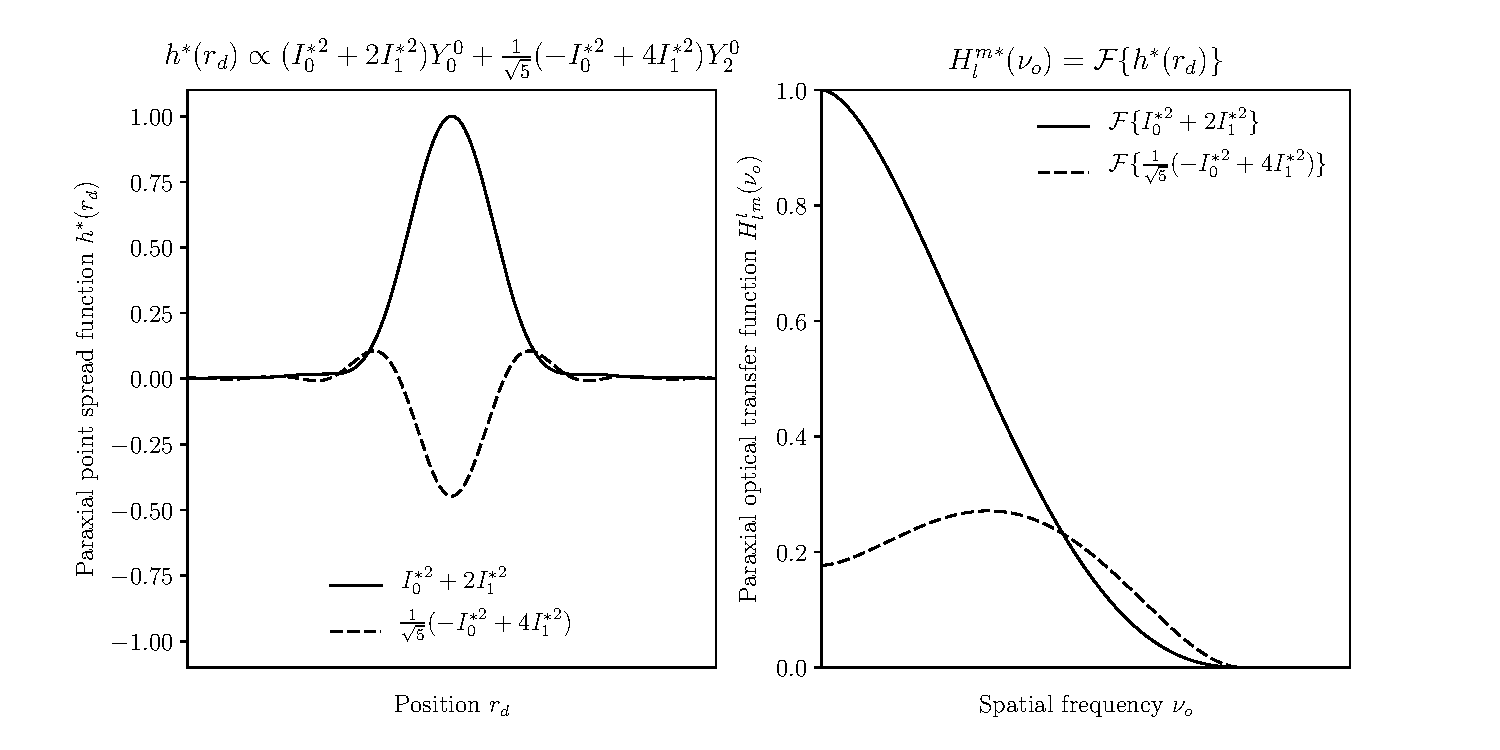
\includegraphics[width = 1.\textwidth]{../calculations/ft.pdf}
   \caption{In progress. \textbf{Left:} Paraxial spatio-angular point spread
     function for a single-view fluorescence microscope with NA=0.8. The solid
     line is the PSF for $y_0^0$ distributions and the dashed line is the PSF
     for $y_2^0$ distributions. $y_2^0$ includes ``negative'' fluorophores, so
     it gives rise to a negative PSF. \textbf{Right:} Numerical paraxial
     spatio-angular optical transfer function for the same microscope. The
     $y_0^0$ term has a spatial low-pass response while the $y_2^0$ term has a
     spatial high-pass response. The relative sizes of the two terms is set by
     the NA---increasing the NA increases the relative size of the $y_0^2$ term.
     Vertical scaling is correct---horizontal scaling is in progress. The cutoff
     frequency is proportional to NA and is the same for both spherical harmonic
     terms.}
   \label{fig:para}
\end{figure}
    
\section{Conclusions}

TODO 

\bibliography{report}{}
\bibliographystyle{unsrt}

\appendix
\section{Products of real spherical harmonics}\label{realspherical}
The six products of $l=1$ spherical harmonics are
\begin{align}
y_1^{-1}y_1^{-1}\sqrt{\pi} &= \frac{1}{2 }y_0^0 - \frac{\sqrt{5}}{10 }y_2^0 - \frac{\sqrt{15}}{10 }y_2^2,\\ 
y_1^{-1}y_1^0\sqrt{\pi} &= \frac{\sqrt{15}}{10 }y_2^{-1} ,\\
y_1^{-1}y_1^1\sqrt{\pi} &= - \frac{\sqrt{15}}{10 }y_2^{-2} ,\\
y_1^0y_1^0\sqrt{\pi} &= \frac{1}{2 }y_0^0 + \frac{\sqrt{5}}{5 }y_2^0 ,\\
y_1^0y_1^1\sqrt{\pi} &= \frac{\sqrt{15}}{10 }y_2^1 ,\\
y_1^1y_1^1\sqrt{\pi} &= \frac{1}{2 }y_0^0 - \frac{\sqrt{5}}{10 }y_2^0 + \frac{\sqrt{15}}{10 }y_2^2.
\end{align}
The fifteen products of $l=2$ spherical harmonics are
\begin{align}
y_2^{-2}y_2^{-2}\sqrt{\pi} &= \frac{1}{2 }y_0^{0} - \frac{\sqrt{5}}{7 }y_2^{0} + \frac{1}{14 }y_4^{0} - \frac{\sqrt{35}}{14 }y_4^{4} \\
y_2^{-2}y_2^{-1}\sqrt{\pi} &= - \frac{\sqrt{15}}{14 }y_2^{1} + \frac{\sqrt{10}}{28 }y_4^{1} + \frac{\sqrt{70}}{28 }y_4^{3} \\
y_2^{-2}y_2^{0}\sqrt{\pi} &= - \frac{\sqrt{5}}{7 }y_2^{-2} + \frac{\sqrt{15}}{14 }y_4^{-2} \\
y_2^{-2}y_2^{1}\sqrt{\pi} &= - \frac{\sqrt{15}}{14 }y_2^{-1} - \frac{\sqrt{70}}{28 }y_4^{-3} + \frac{\sqrt{10}}{28 }y_4^{-1} \\
y_2^{-2}y_2^{2}\sqrt{\pi} &= \frac{\sqrt{35}}{14 }y_4^{-4} \\
y_2^{-1}y_2^{-1}\sqrt{\pi} &= \frac{1}{2 }y_0^{0} + \frac{\sqrt{5}}{14 }y_2^{0} - \frac{\sqrt{15}}{14 }y_2^{2} - \frac{2}{7 }y_4^{0} - \frac{\sqrt{5}}{7 }y_4^{2} \\
y_2^{-1}y_2^{0}\sqrt{\pi} &= \frac{\sqrt{5}}{14 }y_2^{-1} + \frac{\sqrt{30}}{14 }y_4^{-1} \\
y_2^{-1}y_2^{1}\sqrt{\pi} &= - \frac{\sqrt{15}}{14 }y_2^{-2} - \frac{\sqrt{5}}{7 }y_4^{-2} \\
y_2^{-1}y_2^{2}\sqrt{\pi} &= - \frac{\sqrt{15}}{14 }y_2^{-1} + \frac{\sqrt{70}}{28 }y_4^{-3} + \frac{\sqrt{10}}{28 }y_4^{-1} \\
y_2^{0}y_2^{0}\sqrt{\pi} &= \frac{1}{2 }y_0^{0} + \frac{\sqrt{5}}{7 }y_2^{0} + \frac{3}{7 }y_4^{0} \\
y_2^{0}y_2^{1}\sqrt{\pi} &= \frac{\sqrt{5}}{14 }y_2^{1} + \frac{\sqrt{30}}{14 }y_4^{1} \\
y_2^{0}y_2^{2}\sqrt{\pi} &= - \frac{\sqrt{5}}{7 }y_2^{2} + \frac{\sqrt{15}}{14 }y_4^{2} \\
y_2^{1}y_2^{1}\sqrt{\pi} &= \frac{1}{2 }y_0^{0} + \frac{\sqrt{5}}{14 }y_2^{0} + \frac{\sqrt{15}}{14 }y_2^{2} - \frac{2}{7 }y_4^{0} + \frac{\sqrt{5}}{7 }y_4^{2} \\
y_2^{1}y_2^{2}\sqrt{\pi} &= \frac{\sqrt{15}}{14 }y_2^{1} - \frac{\sqrt{10}}{28 }y_4^{1} + \frac{\sqrt{70}}{28 }y_4^{3} \\
y_2^{2}y_2^{2}\sqrt{\pi} &= \frac{1}{2 }y_0^{0} - \frac{\sqrt{5}}{7 }y_2^{0} + \frac{1}{14 }y_4^{0} + \frac{\sqrt{35}}{14 }y_4^{4}
\end{align}

\section{Paraxial coherent transfer function}\label{paraxialctf}
In this appendix we calculate the paraxial CTF for a single-view fluorescence
microscope. We start by plugging Eq. \ref{eq:paracsf} (the paraxial CSF) into Eq.
\ref{eq:csfdef2}
\begin{align}
  {\mb{E}_l^m}^{(p)}(\bs{\nu}) \propto \int_{\mathbb{S}^2}d\so{}\int_{\mathbb{R}^2}d\rd{}'\,
\begin{bmatrix}
    A^{(p)}(r_d')y_1^{1}(\so{}) + 2iB^{(p)}(r_d')\cos\phi_d'y_1^{0}(\so{})\\
    A^{(p)}(r_d')y_1^{-1}(\so{}) + 2iB^{(p)}(r_d')\sin\phi_d'y_1^{0}(\so{})\\
    0\\
  \end{bmatrix}
  y_l^m(\so{})\thinspace\me^{-i 2\pi\rd{}'\cdot\bs{\nu}}. 
\end{align}
We split the integral into two parts by writing
\begin{align}
  {\mb{E}_l^m}^{(p)}(\bs{\nu}) &\propto \int_{\mathbb{S}^2}d\so{}\, \mb{E}^{(p)}(\bs{\nu};\so{}) y_l^m(\so{}),\\ \label{eq:splitup}
  \mb{E}^{(p)}(\bs{\nu};\so{}) &\equiv  \int_{\mathbb{R}^2}d\rd{}'\
\begin{bmatrix}
    A^{(p)}(r_d')y_1^{1}(\so{}) + 2iB^{(p)}(r_d')\cos\phi_d'y_1^{0}(\so{})\\
    A^{(p)}(r_d')y_1^{-1}(\so{}) + 2iB^{(p)}(r_d')\sin\phi_d'y_1^{0}(\so{})\\
    0\\
  \end{bmatrix}
  \thinspace\me^{-i 2\pi\rd{}'\cdot\bs{\nu}}. 
\end{align}
Substituting $A^{(p)}(r_d')$ and $B^{(p)}(r_d')$ using Eq. \ref{eq:abparadef} gives
\begin{align}
  \mb{E}^{(p)}(\bs{\nu}; \so{}) = \int_{\mathbb{R}^2}d\rd{}'\,
\begin{bmatrix}
    \frac{J_1(2\pi ar_d')}{\pi ar_d'}y_1^m(\so{}) + 2i\frac{\text{NA}}{n_o}\left[\frac{J_2(2\pi ar_d')}{\pi ar_d'}\right]\cos\phi_d'y_1^0(\so{})\\
    \frac{J_1(2\pi ar_d')}{\pi ar_d'}y_1^{-1}(\so{}) + 2i\frac{\text{NA}}{n_o}\left[\frac{J_2(2\pi ar_d')}{\pi ar_d'}\right]\sin\phi_d'y_1^0(\so{})\\
    0\\
  \end{bmatrix}
  \thinspace\me^{-i 2\pi\rd{}'\cdot\bs{\nu}}.
\end{align}
We can rewrite this in terms of three two-dimensional Fourier transforms
\begin{align}
  \mb{E}^{(p)}(\bs{\nu}; \so{}) \propto 
\begin{bmatrix}
    t_1(\bs{\nu})y_1^1(\so{}) + t_2(\bs{\nu})y_1^0(\so{})\\
    t_1(\bs{\nu})y_1^{-1}(\so{}) + t_3(\bs{\nu})y_1^0(\so{})\\
    0\\
  \end{bmatrix}\label{eq:tint}
\end{align}
where
\begin{align}
  t_1(\bs{\nu}) &\equiv \frac{1}{\pi a}\int_{\mathbb{R}^2}d\rd{}'\,  \frac{J_1(2\pi ar_d')}{r_d'}\, \me^{-i 2\pi\rd{}'\cdot\bs{\nu}},\\
  t_2(\bs{\nu}) &\equiv \frac{2i}{\pi a}\frac{\text{NA}}{n_o}\int_{\mathbb{R}^2}d\rd{}'\, \frac{J_2(2\pi ar_d')}{r_d'}\cos\phi_d'\, \me^{-i 2\pi\rd{}'\cdot\bs{\nu}},\\
  t_3(\bs{\nu}) &\equiv \frac{2i}{\pi a}\frac{\text{NA}}{n_o}\int_{\mathbb{R}^2}d\rd{}'\, \frac{J_2(2\pi ar_d')}{r_d'}\sin\phi_d'\, \me^{-i 2\pi\rd{}'\cdot\bs{\nu}}.
\end{align}
All three of the functions to be transformed are separable in polar coordinates,
so we can rewrite the Fourier transform as a sum of weighted Hankel transforms
\cite{goodman1996}. In general, if a function $g(r, \theta)$ is separable in
polar coordinates then we can rewrite it as
$g(r, \theta) = g_{R}(r)g_{\Theta}(\theta)$ and its two-dimensional Fourier transform
is given by
\begin{align}
  \mathcal{F}\{g(r, \theta)\} = \sum_{k=-\infty}^{\infty}c_k(-i)^k\me^{ik\phi}\mathcal{H}_k\{g_R(r)\}
\end{align}
where
\begin{align}
  c_k = \frac{1}{2\pi}\int_0^{2\pi}d\theta\, g_{\Theta}(\theta)\me^{-ik\theta}
\end{align}
and $\mathcal{H}_k\{\}$ is the Hankel transform of order $k$ given by
\begin{align}
  \mathcal{H}_k\{g_R(r)\} = 2\pi\int_0^{\infty}dr\, r g_R(r)J_k(2\pi r \nu).
\end{align}
First, we evaluate $t_1(\bs{\nu})$. The Fourier transform will be in polar
coordinates, so we define polar coordinates in frequency space as
$\bs{\nu} \equiv \nu\cos\phi_\nu\mh{x} + \nu\sin\phi_\nu\mh{y} \equiv \nu_x\mh{x} + \nu_y\mh{y}$. The
angular part of $J_z(ar_d')/r_d'$ is a constant, so $c_k = \delta(k)$ which
means we only need to evaluate the zero-order Hankel transform
\begin{align}
  t_1(\bs{\nu}) = \frac{1}{\pi a}\mathcal{H}_0\left\{\frac{J_1(2\pi ar_d')}{r_d'}\right\}.
\end{align}
From tabulated Hankel transforms we find that
\begin{align}
  \mathcal{H}_{\mu}\left\{\frac{J_{\mu+1}(2\pi ar_d')}{r_d'}\right\} =
  \frac{1}{2\pi}a^{-\mu-1}\nu^\mu\, \Pi\left(\frac{\nu}{a}\right)\label{eq:hankstar}
\end{align}
when $a > 0$ and $\text{Re}(\mu) > -\frac{3}{2}$ \cite{poul1998}. Applying this result
we find that
\begin{align}
  t_1(\bs{\nu}) =
    \frac{1}{2\pi^2 a^{2}}\, \Pi\left(\frac{\nu}{a}\right)\label{eq:t1final}.
\end{align}
To evaluate $t_2(\bs{\nu})$ and $t_3(\bs{\nu})$ we need to be careful with the angular part. For $t_2(\bs{\nu})$
the angular part of the function is $\cos\phi_d' = \frac{1}{2}\left(e^{i\phi_d'} + e^{-i\phi_d'}\right)$. Therefore, $c_k = \frac{1}{2}\delta(k-1) + \frac{1}{2}\delta(k+1)$ and we have to evaluate two Hankel transforms given by
\begin{align}
  t_2(\bs{\nu}) = \frac{2i}{\pi a}\frac{\text{NA}}{n_o}\left[ie^{-i\phi_{\nu}}\mathcal{H}_{-1}\left\{\frac{J_2(2\pi ar_d')}{\pi ar_d'}\right\} - ie^{i\phi_{\nu}}\mathcal{H}_{1}\left\{\frac{J_2(2\pi ar_d')}{\pi ar_d'}\right\}\right].
\end{align}
To put the Hankel transforms in the form of Eq. \ref{eq:hankstar} we apply
$\mathcal{H}_\mu = (-1)^\mu\mathcal{H}_{-\mu}$ to get
\begin{align}
  t_2(\bs{\nu}) = \frac{2i}{\pi a}\frac{\text{NA}}{n_o}\left[-ie^{-i\phi_{\nu}}\mathcal{H}_{1}\left\{\frac{J_2(2\pi ar_d')}{\pi ar_d'}\right\} - ie^{i\phi_{\nu}}\mathcal{H}_{1}\left\{\frac{J_2(2\pi ar_d')}{\pi ar_d'}\right\}\right].
\end{align}
Applying Eq. \ref{eq:hankstar} and simplifying gives
\begin{align}
  t_2(\bs{\nu}) =
    \frac{1}{\pi^2 a^3}\frac{\text{NA}}{n_o}\nu(e^{-i\phi_\nu} + e^{i\phi_\nu})\, \Pi\left(\frac{\nu}{a}\right)
\end{align}
Finally, 
\begin{align}
  t_2(\bs{\nu}) =
    \frac{1}{\pi^2 a^3}\frac{\text{NA}}{n_o}\nu\cos\phi_{\nu}\, \Pi\left(\frac{\nu}{a}\right)\label{eq:t2final}
\end{align}
Similarly, 
\begin{align}
  t_3(\bs{\nu}) =
    \frac{1}{\pi^2 a^3}\frac{\text{NA}}{n_o}\nu\sin\phi_{\nu}\, \Pi\left(\frac{\nu}{a}\right)\label{eq:t3final}
\end{align}
Plugging Eqs. \ref{eq:t1final}, \ref{eq:t2final}, and \ref{eq:t3final} into Eq.
\ref{eq:tint} and normalizing gives
\begin{align}
  {\mb{E}}^{(p)}(\bs{\nu}; \so{}) =
\begin{bmatrix}
  y_1^1(\so{}) + \frac{2}{a}\frac{\text{NA}}{n_o}\nu\cos\phi_\nu y_1^0(\so{})\\
  y_1^{-1}(\so{}) + \frac{2}{a}\frac{\text{NA}}{n_o}\nu\sin\phi_\nu y_1^0(\so{})\\
  0\\
  \end{bmatrix}\, \Pi\left(\frac{\nu}{a}\right). \label{eq:paractfsp}
\end{align}
Finally, we find the paraxial CTF by evaluating the angular integral in Eq.
\ref{eq:splitup} 
\begin{align}
  {\mb{E}_l^m}^{(p)}(\bs{\nu}) =
\begin{bmatrix}
  \delta(l-1, m-1) + \frac{2}{a}\frac{\text{NA}}{n_o}\nu\cos\phi_\nu\delta(l-1, m)\\
  \delta(l-1, m+1) + \frac{2}{a}\frac{\text{NA}}{n_o}\nu\sin\phi_\nu\delta(l-1, m)\\
  0\\
  \end{bmatrix}\, \Pi\left(\frac{\nu}{a}\right).
\end{align}

\section{Paraxial optical transfer function}\label{paraxialotf}
In this appendix we calculate the paraxial OTF for a single-view fluorescence
microscope. We start with Eq. \ref{eq:otfdef2}
\begin{align}
  H_l^m(\bs{\nu}) \propto \int_{\mathbb{S}^2}d\so{}\int_{\mathbb{R}^2}d\rd{}'\, h(\rd{}', \so{}) y_l^m(\so{})\thinspace\me^{-i 2\pi \rd{}'\cdot\bs{\nu}}.\label{eq:otfdef2}
\end{align}
We could plug in the paraxial PSF and evaluate the integrals, but this will lead
us to Fourier transforms that cannot be found in tables. Instead we use a trick
from scalar Fourier optics and write the OTF in terms of the detected electric
field \cite{goodman1996}
\begin{align}
  H_l^m(\bs{\nu}) \propto \int_{\mathbb{S}^2}d\so{}\int_{\mathbb{R}^2}d\rd{}'\, \left|\mb{e}_d(\rd{}', \so{})\right|^2 y_l^m(\so{})\thinspace\me^{-i 2\pi \rd{}'\cdot\bs{\nu}}.
\end{align}
Next, we manipulate this equation to
\begin{align}
  H_l^m(\bs{\nu}) &\propto \int_{\mathbb{S}^2}d\so{}\, y_l^m(\so{})\int_{\mathbb{R}^2}d\rd{}'\, \mb{e}^{\dagger}_d(\rd{}', \so{})\mb{e}_d(\rd{}', \so{})\, \me^{-i 2\pi \rd{}'\cdot\bs{\nu}},\\
  H_l^m(\bs{\nu}) &\propto \int_{\mathbb{S}^2}d\so{}\, y_l^m(\so{})\int_{\mathbb{R}^2}d\rd{}'\, \int_{\mathbb{R}^2}d\rd{}''\, \mb{e}^{\dagger}_d(\rd{}', \so{})\mb{e}_d(\rd{}'', \so{})\delta(\rd{}'' - \rd{}')\, \me^{-i 2\pi \rd{}''\cdot\bs{\nu}},\\
  H_l^m(\bs{\nu}) &\propto \int_{\mathbb{S}^2}d\so{}\, y_l^m(\so{})\int_{\mathbb{R}^2}d\bs{\tau}\,\int_{\mathbb{R}^2}d\rd{}'\, \int_{\mathbb{R}^2}d\rd{}''\, \mb{e}^{\dagger}_d(\rd{}', \so{})\mb{e}_d(\rd{}'', \so{})\me^{-i 2\pi\bs{\tau}(\rd{}'' - \rd{}')}\me^{-i 2\pi \rd{}''\cdot\bs{\nu}},\\
  H_l^m(\bs{\nu}) &\propto \int_{\mathbb{S}^2}d\so{}\, y_l^m(\so{})\int_{\mathbb{R}^2}d\bs{\tau}\,\left[\int_{\mathbb{R}^2}d\rd{}'\, \mb{e}^{\dagger}_d(\rd{}', \so{}) \me^{i 2\pi\rd{}'\cdot \bs{\nu}}\right]\left[\int_{\mathbb{R}^2}d\rd{}''\, \mb{e}_d(\rd{}'', \so{})\me^{-i 2\pi \rd{}''\cdot(\bs{\nu} + \bs{\tau})}\right],\\
  H_l^m(\bs{\nu}) &\propto \int_{\mathbb{S}^2}d\so{}\, y_l^m(\so{})\int_{\mathbb{R}^2}d\bs{\tau}\,\mb{E}^{\dagger}(\bs{\tau}; \so{})\mb{E}(\bs{\tau} + \bs{\nu}; \so{}). \label{eq:hlmauto}
\end{align}
We have followed the proof for the Wiener-Kinchin theorem \cite{papoulis2002, wiener} to explicitly show how the angular integral affects the usual scalar
calculation. Eq. \ref{eq:hlmauto} shows that we can calculate the OTF by taking
the vector autocorrelation of the spatial CTF then projecting the result onto
the spherical harmonics.

We will rewrite Eq. \ref{eq:hlmauto} in two parts
\begin{align}
  H_l^m(\bs{\nu}) &\propto \int_{\mathbb{S}^2}d\so{}\, y_l^m(\so{}) H(\bs{\nu}; \so{})  \label{eq:hlmauto2}\\
  H(\bs{\nu}; \so{}) &\equiv \int_{\mathbb{R}^2}d\bs{\tau}\,\mb{E}^{\dagger}(\bs{\tau}- \bs{\nu}/2; \so{})\mb{E}(\bs{\tau} + \bs{\nu}/2; \so{}). \label{eq:hlmspatial}
\end{align}
Notice the change of variable to simplify the autocorrelation. In the previous
section we calculated the CTF in the paraxial case as 
\begin{align}
  {\mb{E}}^{(p)}(\bs{\nu}; \so{}) =
\begin{bmatrix}
  y_1^1(\so{}) + \frac{2}{a}\frac{\text{NA}}{n_o}\nu\cos\phi_\nu y_1^0(\so{})\\
  y_1^{-1}(\so{}) + \frac{2}{a}\frac{\text{NA}}{n_o}\nu\sin\phi_\nu y_1^0(\so{})\\
  0\\
  \end{bmatrix}\, \Pi\left(\frac{\nu}{a}\right). \label{eq:ctfparax}
\end{align}
By introducing $\bs{\tau} \equiv \tau_x\mh{x} + \tau_y\mh{y} \equiv \tau\cos\phi_\tau\mh{x} + \tau\sin\phi_\tau\mh{y}$
we can plug Eq. \ref{eq:ctfparax} into Eq. \ref{eq:hlmspatial} and find that
\begin{align}
    H^{(p)}(\bs{\nu}; \so{}) = \int_{\mathbb{R}^2}d\bs{\tau}\, &\begin{bmatrix}
  y_1^1(\so{}) + \frac{2}{a}\frac{\text{NA}}{n_o}(\tau_x - \frac{1}{2}\nu_x) y_1^0(\so{})\\
  y_1^{-1}(\so{}) + \frac{2}{a}\frac{\text{NA}}{n_o}(\tau_y - \frac{1}{2}\nu_y) y_1^0(\so{})\\
  0\\
\end{bmatrix}^{\dagger}
  \begin{bmatrix}
  y_1^1(\so{}) + \frac{2}{a}\frac{\text{NA}}{n_o}(\tau_x + \frac{1}{2}\nu_x) y_1^0(\so{})\\
  y_1^{-1}(\so{}) + \frac{2}{a}\frac{\text{NA}}{n_o}(\tau_y + \frac{1}{2}\nu_y) y_1^0(\so{})\\
  0\\
\end{bmatrix}\nonumber \\
  &\Pi\left(\frac{\tau - \nu/2}{a}\right)\Pi\left(\frac{\tau + \nu/2}{a}\right).
\end{align}
Expanding the inner product gives
\begin{align}
    H^{(p)}(\bs{\nu}; \so{}) = \int_{\mathbb{R}^2}d\bs{\tau}\, &
      \{y_1^1(\so{})\}^2  + \left\{\frac{2}{a}\frac{\text{NA}}{n_o}y_1^0(\so{})\right\}^2(\tau_x - \frac{1}{2}\nu_x)(\tau_x + \frac{1}{2}\nu_x) + \nonumber \\
                                                                 &\{y_1^{-1}(\so{})\}^2 + \left\{\frac{2}{a}\frac{\text{NA}}{n_o}y_1^0(\so{})\right\}^2(\tau_y - \frac{1}{2}\nu_y)(\tau_y + \frac{1}{2}\nu_y) + \nonumber \\
                                                                 &\left\{\frac{2}{a}\frac{\text{NA}}{n_o}y_1^0(\so{})y_1^1(\so{})\right\}(\tau_x - \frac{1}{2}\nu_x) + \left\{\frac{2}{a}\frac{\text{NA}}{n_o}y_1^0(\so{})y_1^1(\so{})\right\}(\tau_x + \frac{1}{2}\nu_x) \nonumber \\
  &\left\{\frac{2}{a}\frac{\text{NA}}{n_o}y_1^0(\so{})y_1^{-1}(\so{})\right\}(\tau_y - \frac{1}{2}\nu_y) + \left\{\frac{2}{a}\frac{\text{NA}}{n_o}y_1^0(\so{})y_1^{-1}(\so{})\right\}(\tau_y + \frac{1}{2}\nu_y) \nonumber \\  
&\Pi\left(\frac{\tau - \nu/2}{a}\right)\Pi\left(\frac{\tau + \nu/2}{a}\right). 
\end{align}
All of the terms with a single $\tau_x$ or $\tau_y$ are odd, so they integrate
to zero. Therefore
\begin{align}
    H^{(p)}(\bs{\nu}; \so{}) = \int_{\mathbb{R}^2}d\bs{\tau}\, &
      \{y_1^1(\so{})\}^2  + \left\{\frac{2}{a}\frac{\text{NA}}{n_o}y_1^0(\so{})\right\}^2(\tau_x - \frac{1}{2}\nu_x)(\tau_x + \frac{1}{2}\nu_x) + \nonumber \\
                                                                 &\{y_1^{-1}(\so{})\}^2 + \left\{\frac{2}{a}\frac{\text{NA}}{n_o}y_1^0(\so{})\right\}^2(\tau_y - \frac{1}{2}\nu_y)(\tau_y + \frac{1}{2}\nu_y) + \nonumber \\
&\Pi\left(\frac{\tau - \nu/2}{a}\right)\Pi\left(\frac{\tau + \nu/2}{a}\right). 
\end{align}
After expanding the spherical harmonics we can rewrite this equation in terms of
three autocorrelations
\begin{align}
    H^{(p)}(\bs{\nu}; \so{}) &= [s_1(\bs{\nu}) + s_2(\bs{\nu}) + s_3(\bs{\nu})]y_0^0(\so{}) + \frac{2\text{NA}}{\sqrt{5}a n_o}[-s_1(\bs{\nu}) + s_2(\bs{\nu}) + s_3(\bs{\nu})]y_2^0(\so{})\label{eq:hinter}
\end{align}
where
\begin{align}
  s_1(\bs{\nu}) &\equiv \int_{\mathbb{R}^2}d\bs{\tau}\, \Pi\left(\frac{\tau - \nu/2}{a}\right)\Pi\left(\frac{\tau + \nu/2}{a}\right),\\
  s_2(\bs{\nu}) &\equiv \int_{\mathbb{R}^2}d\bs{\tau}\, (\tau_x - \nu_x/2)(\tau_x + \nu_x/2) \Pi\left(\frac{\tau - \nu/2}{a}\right)\Pi\left(\frac{\tau + \nu/2}{a}\right),\\
  s_3(\bs{\nu}) &\equiv \int_{\mathbb{R}^2}d\bs{\tau}\, (\tau_y - \nu_y/2)(\tau_y + \nu_y/2) \Pi\left(\frac{\tau - \nu/2}{a}\right)\Pi\left(\frac{\tau + \nu/2}{a}\right).
\end{align}
We can evaluate these integrals with the help of the geometric construction
shown in Figure \ref{fig:geometry} \cite{goodman1996}. 

\begin{figure}[h]
 \captionsetup{width=1.0\linewidth}
 \centering
   \centering
   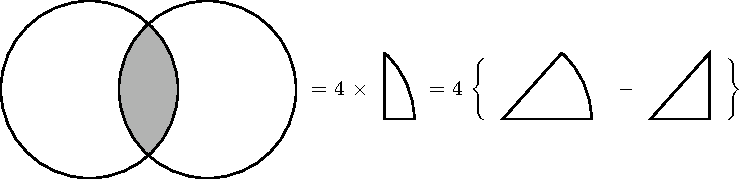
\includegraphics[width = 0.8\textwidth]{../figures/geometry/geometry.pdf}
   \caption{Geometric construction for evaluating $s_1(\bs{\nu})$,
     $s_2(\bs{\nu})$, and $s_3(\bs{\nu})$. We need to find the boundaries of
     integration for the overlapping region of two circles with radius $a$ and
     distance $\nu$ between their centers. The region is given by four times the
     difference in area between a sector of angle
     $\arccos\left(\frac{\nu}{2a}\right)$ and a triangle with base $\nu/2$ and
     hypotenuse $a$.}
   \label{fig:geometry}
\end{figure}

Starting with $s_1(\bs{\nu})$ we find that
\begin{align}
  s_1(\bs{\nu}) &= 4\left[\left(\int\limits_0^a d\tau\, \tau\int\limits_0^{\arccos\left(\frac{\nu}{2a}\right)}d\phi_{\tau}\right) - \left(\int\limits_0^{\nu/2}d\tau_x \int\limits_0^{\tau_x\frac{2a}{\nu}\sqrt{1 - \left(\frac{\nu}{2a}\right)^2}}d\tau_y\right)\right]\\
  s_1(\bs{\nu}) &= 4\left[\left(\int\limits_0^a d\tau\,\tau\arccos\left(\frac{\nu}{2a}\right)\right) - \left(\int\limits_0^{\nu/2}d\tau_x \tau_x \frac{2a}{\nu}\sqrt{1 - \left(\frac{\nu}{2a}\right)^2}\right)\right]\\
  s_1(\bs{\nu}) &= 4\left[\frac{a^2}{2}\arccos\left(\frac{\nu}{2a}\right) - \frac{\nu a}{4}\sqrt{1 - \left(\frac{\nu}{2a}\right)^2}\right]\\
  s_1(\bs{\nu}) &= 2a^2\arccos\left(\frac{\nu}{2a}\right) - \nu a\sqrt{1 - \left(\frac{\nu}{2a}\right)^2}.
\end{align}
Note that $s_1(\bs{\nu})$ is the unnormalized OTF for a single-view
fluorescence microscope under the scalar approximation. Next we evaluate
$s_2(\bs{\nu})$ using the same geometric construction. This integral is not
rotationally symmetric, so we start by restricting $\bs{\nu}$ to the $x$-axis
\begin{align}
  s_2(\nu_x) = 4\Bigg[&\int\limits_0^a d\tau\, \tau \int\limits_0^{\arccos\left(\frac{\nu_x}{2a}\right)}d\phi_{\tau}(\tau\cos\phi_{\tau} - \nu_x/2)(\tau\cos\phi_{\tau} + \nu_x/2)\nonumber \\ &- \int\limits_0^{\nu_x/2}d\tau_x \int\limits_0^{\tau_x \frac{2a}{\nu_x}\sqrt{1 - \left(\frac{\nu_x}{2a}\right)^2}}d\tau_y(\tau_x - \nu_x/2)(\tau_x + \nu_x/2)\Bigg],\\
  s_2(\nu_x) = 4\Bigg[&\int\limits_0^a d\tau\, \tau\int\limits_0^{\arccos\left(\frac{\nu_x}{2a}\right)}d\phi_{\tau}(\tau^2\cos^2\phi_{\tau} - \nu_x^2/4)\nonumber \\ &- \int\limits_0^{\nu_x/2}d\tau_x \int\limits_0^{\tau_x\frac{2 a}{\nu_x}\sqrt{1 - \left(\frac{\nu_x}{2a}\right)^2}}d\tau_y(\tau_x^2 - \nu_x^2/4)\Bigg].
\end{align}
For the first inner integral we will make use of the following
\begin{align}
  \int\limits_0^{\arccos(z)} d\phi \cos^2\phi = \frac{1}{2}z\sqrt{1 - z^2} + \frac{1}{2}\arccos(z).
\end{align}
This results in
\begin{align}
  s_2(\nu_x) = 4\Bigg[&\int\limits_0^a d\tau\left(\frac{\tau^3}{2}\left(\frac{\nu_x}{2a}\right)\sqrt{1 - \left(\frac{\nu_x}{2a}\right)^2} + \frac{\tau^3}{2}\arccos\left(\frac{\nu_x}{2a}\right) - \frac{\tau\nu_x^2}{4}\arccos\left(\frac{\nu_x}{2a}\right)\right)\nonumber \\ &- \int\limits_0^{\nu_x/2}d\tau_x \left(\tau_x^3 - \frac{\tau_x\nu_x^2}{4}\right)\frac{2 a}{\nu_x}\sqrt{1 - \left(\frac{\nu_x}{2a}\right)^2}\Bigg],\\
  s_2(\nu_x) = 4\Bigg[&\left(\frac{a^4}{8}\left(\frac{\nu_x}{2a}\right)\sqrt{1 - \left(\frac{\nu_x}{2a}\right)^2} + \frac{a^4}{8}\arccos\left(\frac{\nu_x}{2a}\right) - \frac{a^2\nu_x^2}{8}\arccos\left(\frac{\nu_x}{2a}\right)\right) - \left(\frac{\nu_x^4}{64} - \frac{\nu_x^4}{32}\right)\frac{2 a}{\nu_x}\sqrt{1 - \left(\frac{\nu_x}{2a}\right)^2}\Bigg],\\
  s_2(\nu_x) = 4\Bigg[&\frac{\nu_xa^3}{16}\sqrt{1 - \left(\frac{\nu_x}{2a}\right)^2} + \frac{a^4}{8}\arccos\left(\frac{\nu_x}{2a}\right) - \frac{a^2\nu_x^2}{8}\arccos\left(\frac{\nu_x}{2a}\right) + \frac{\nu_x^3a}{32}\sqrt{1 - \left(\frac{\nu_x}{2a}\right)^2}\Bigg],\\
  s_2(\nu_x) = &\frac{\nu_xa^3}{4}\sqrt{1 - \left(\frac{\nu_x}{2a}\right)^2} + \frac{a^4}{2}\arccos\left(\frac{\nu_x}{2a}\right) - \frac{a^2\nu_x^2}{2}\arccos\left(\frac{\nu_x}{2a}\right) + \frac{\nu_x^3a}{8}\sqrt{1 - \left(\frac{\nu_x}{2a}\right)^2},\\
  s_2(\nu_x) = &\left(\frac{a^2}{4} - \frac{\nu_x^2}{4}\right)2a^2\arccos\left(\frac{\nu_x}{2a}\right) + \left(\frac{a^2}{4} + \frac{\nu_x^2}{8}\right)\nu_x a \sqrt{1 - \left(\frac{\nu_x}{2a}\right)^2}.
\end{align}
This result is only true for $\bs{\nu}$ restricted to the $x$ axis, but we can
extend this result to the general case by noticing that the value of the
function in the area of overlap has the same functional form for any direction
of $\bs{\nu}$ but the total value is reduced by a factor of $\cos^2\phi_\nu$.
This make sense because the function in the area of overlap for the circles
displaced along the $y$-axis is zero. Therefore, the complete integral is given
by 
\begin{align}
    s_2(\bs{\nu}) = &\cos^2\phi_\nu\left[\left(\frac{a^2}{4} - \frac{\nu^2}{4}\right)2a^2\arccos\left(\frac{\nu}{2a}\right) + \left(\frac{a^2}{4} + \frac{\nu^2}{8}\right)\nu a\sqrt{1 - \left(\frac{\nu}{2a}\right)^2}\right].
\end{align}
Similarly, $s_3(\bs{\nu})$ is given by
\begin{align}
      s_3(\bs{\nu}) = &\sin^2\phi_\nu\left[\left(\frac{a^2}{4} - \frac{\nu^2}{4}\right)2a^2\arccos\left(\frac{\nu}{2a}\right) + \left(\frac{a^2}{4} + \frac{\nu^2}{8}\right)\nu a\sqrt{1 - \left(\frac{\nu}{2a}\right)^2}\right].
\end{align}
Plugging these results into Eq. \ref{eq:hinter} gives
\begin{align}
    H^{(p)}(\bs{\nu}; \so{}) = &\left[\left(1 + \frac{a^2}{4} - \frac{\nu^2}{4}\right)2a^2\arccos\left(\frac{\nu}{2a}\right) - \left(1 - \frac{a^2}{4} - \frac{\nu^2}{8}\right)\nu a\sqrt{1 - \left(\frac{\nu}{2a}\right)^2}\right]y_0^0(\so{})\nonumber\\ + &\left[\left(-1 + \frac{a^2}{4} - \frac{\nu^2}{4}\right)2a^2\arccos\left(\frac{\nu}{2a}\right) - \left(-1 - \frac{a^2}{4} - \frac{\nu^2}{8}\right)\nu a\sqrt{1 - \left(\frac{\nu}{2a}\right)^2}\right]y_2^0(\so{}).
\end{align}
After plugging this into Eq. \ref{eq:hlmauto2}, performing the angular integral,
refactoring, and normalizing, we get the complete spatio-angular transfer function
\begin{align}
  H_l^m(\nu) &= H_0^0(\nu)\delta(l, m) + \frac{2\text{NA}}{\sqrt{5}an_o}H_2^0(\nu)\delta(l-2, m)\\
  H_0^0(\nu) &= \left(1 + \frac{a^2}{4} - \frac{\nu^2}{4}\right)2a^2\arccos\left(\frac{\nu}{2a}\right) - \left(1 - \frac{a^2}{4} - \frac{\nu^2}{8}\right)\nu a\sqrt{1 - \left(\frac{\nu}{2a}\right)^2}\\
  H_2^0(\nu) &= \left(-1 + \frac{a^2}{4} - \frac{\nu^2}{4}\right)2a^2\arccos\left(\frac{\nu}{2a}\right) - \left(-1 - \frac{a^2}{4} - \frac{\nu^2}{8}\right)\nu a\sqrt{1 - \left(\frac{\nu}{2a}\right)^2}               
\end{align}

\end{document}
